\chapter{Praktická část}
\label{5-postup}

\section{Aktualizace pluginu do verze 1.0}
Po dokončení pluginu v předmětu Free Software GIS měl plugin veškerou základní 
funkcionalitu, kterou měl mít. Tou bylo načítání GTFS ZIP souboru do QGISu,
rozbalení ZIP souboru, načtení CSV souborů do geodatabázového kontajneru GeoPackage (dále GPKG),
vytvoření vektorových vrstev pro soubory \textit{stops.txt} a \textit{shapes.txt},
obarvení vektorové vrty \textit{shapes.txt} a vložení do CSV souborů a vrstev do
\textit{layer tree} \footnote{součást QGISu odpovědná za zobrazení seznamu vrstev}.
% vysvětlit layer tree, GeoPackage??

Avšak pro uvedení do "ostrého" provozu musel být plugin více uživatelsky přívětivější.
Proto byl veškerý proces přesunut na pozadí, aby celý QGIS program "nezamrzal" a
mohla se při jeho výpočtech provádět i jiné akce. To se provedlo díky Python třídě \textit{QgsTask}
a jejím metodám, které byly zděděny z této třídy. \cite{QgsTask}
% dát sem i ukázku kódu? 

Pro zobrazování procesu během výpočtu byla použita třída \textit{QProgressBar} a její metody.
Zobrazení postupu bylo implementováno do lišty zpráv QGISu spolu s chybovými hláškami.

\begin{figure}[H] \centering
    
\includegraphics[width=400pt]{./pictures/loading.png}
    \caption[ProgressBar]{ProgressBar v liště QGISu}
	\label{fig:ProgressBar v liště QGISu}              
\end{figure}     

% možná přidat code refactorization

\section{Tvorba vizualizace tarifních pásem (verze 2.0)}

Při myšlenkách, jak se k tvorbě tarifních pásem postavit,
se naskytla možnost to vypracovat pomocí Grafického modeláře, který je zabudovaný v QGISu. 
Kvůli omezeným možnostem úprav nástrojů se z těchto myšlenek upustilo a začal se tvořit postup
na "čístý" Python skript pomocí QGIS nástrojů. I přes to, že lze z Grafického modeláře exportovat skript. 

Pro použití QGIS nástrojů v Python skriptu je potřeba importovat modul \textit{processing},
který má funkci \textit{run}, do které se vkládají dva parametry. První parametr je ID nástroje
ve formě \textit{stringu} a druhý je \textit{slovník} vstupních parametrů. Vstupní parametry se lze dozvědět
z QGIS dokumentace. \cite{QGIS_docs}

\subsection{Dialogové okno pro tvorbu tarifních pásem}

Aby se mohl uživatel mohl rozhodnout při jeho používání pluginu, či chce vytvářet tarifní pásma nebo ne, bylo vytvořeno
dialogové okno pomocí PyQt (viz obrázek \ref{fig:dialog}). Toto dialogové okno se vždy zobrazí po stisknutí tlačítka
\textit{Load} pro načtení GTFS souboru. Jak je v závorce napsáno, tvorba tarifních pásem je zatím jen pro PID\_GTFS.
Tvorba tarifních pásem pro ostatní GTFS soubory může být jako námět pro další závěrečné práce nebo ho mohou dobrovolně
vypracovat uživatelé Githubu.

Ovládání dialogového okna je jednoduché. Disponuje běžnými tlačítky pro minimalizaci okna a vypnutí okna, což mimochodem
zruší kompletně proces načítání GTFS souboru. Mimo to tu jsou dvě tlačítka Yes/No, které buďto povolí vytváření tarifních
pásem anebo nepovolí a proces běží jako ve verzi pluginu 1.0.

\begin{figure}[H] \centering
    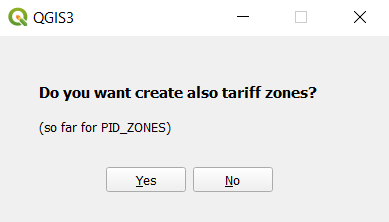
\includegraphics[width=200pt]{./pictures/dialog.png}
    \caption[Dialogové okno s možností tvořit/netvořit tarifní pásma]{Dialogové okno s možností tvořit/netvořit tarifní pásma}
	\label{fig:dialog}                                
\end{figure}

Kvůli přehlednosti byl založen nový Python skript \textit{zones.py} se třídou GtfsZones. Instance této třídy je vytvořena
v hlavním Python skriptu \textit{GTFS.py}.

\subsection{Hrubý tvar tarifních pásem}

GTFS obsahuje povinný CSV soubor \textit{stops.txt} (viz kapitola \ref{stops.txt}). Tento soubor obsahuje mimo
jiných polí také pole \textit{zone\_id}, které bylo při tvorbě tarifních pásem klíčové. 
Pole \textit{zone\_id} má datový typ \textit{string} a znamená, ve kterém tarifním
pásmu daná zastávka leží. Verze GTFS Loaderu 1.0 soubor \textit{stops.txt} převádí do vektorové vrstvy
ve formě bodů. Z této bodové vrstvy byla vytvořena vektorová vrstva Voroného 
diagramů nástrojem \textit{Voroného polygony} v programu QGIS. 

Vstupem do tohoto nástroje je vektorová vrstva stops a výstupem jsou právě Voroného polygony.

\begin{figure}[H] \centering
    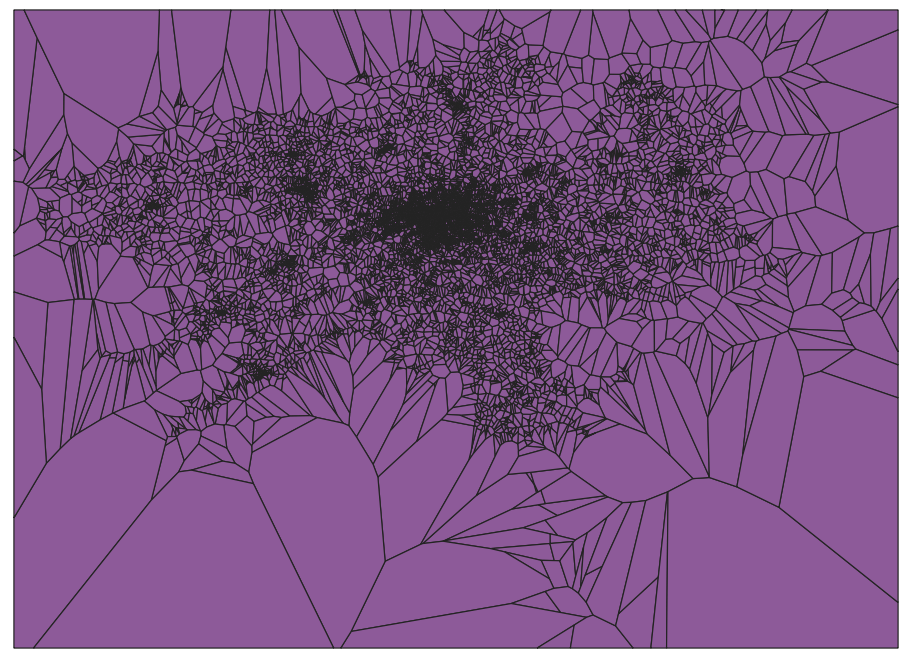
\includegraphics[width=400pt]{./pictures/voronoi-stops.png}
    \caption[Voroného polygony pro všechny zastávky]{Voroného polygony pro všechny zastávky}
	\label{fig:voronoi-stops}              
\end{figure}
  
Pro každé tarifní pásmo byly vybrány zastávky pomocí třídy \textit{QgsVectorLayer}
a její metody \textit{selectByExpression}, která má parametr \textit{expression} ve formě datového
typu \textit{string}. 
Třída \textit{QgsVectorLayer} zároveň vrací vektorovou vrstvu, která může být považována jako vstup do nástroje QGIS.

\subsubsection{Tarifní pásma P, 0 a B}

Speciálně pro tarifní pásma na území Prahy, tedy pro tarifní pásma P, 0 a B byl tvořen rozdílný postup
nežs pro ostatní pásma ležící ve Středních Čechách. Do metody \textit{selectByExpression} byl vložen
parametr s dotazem: 

\["zone\_id"\ IN\ ('P','0','B')\ AND\ "location\_type" = 0\]

Po proběhnutí tohoto dotazu byly vybrány všechny zastávky ležící v tarifních pásmech P, 0 a B. 

V zadávaném výrazu figuruje taktéž údaj o poli \textit{location\_type}, což je typ lokace. 
Hodnota nuly (nebo prázdná hodnota) je právě lokace zastávky viz \ref{stops.txt}.

Některé zastávky se nacházely na stejném a měly duplicitní geometrii, což vytvářelo v dalším
zpracování pouze problém s duplicitními polygony. Aby se takové věci ve výsledku zamezilo, byl použit nástroj   
Delete duplicate geometries, který ve vstupní vektorové vrstvě najde duplicitní geometrie a smaže je.

Pro vybrané zastávky bylo potřeba vybrat ty Voroného polygony, které svou
pozicí dané zastávky protínaly. To bylo provedeno nástrojem \textit{Select by location},
do kterého vstupovala vrstva vybraných zastávek a vrstva Voroného polygonů. Výsledkem tohoto nástroje byla
vektorová vrstva vybraných Voroného polygonů. Jako příklad v obrázku zde budu uvádět tarifní pásmo 2.

\begin{figure}[H] \centering
    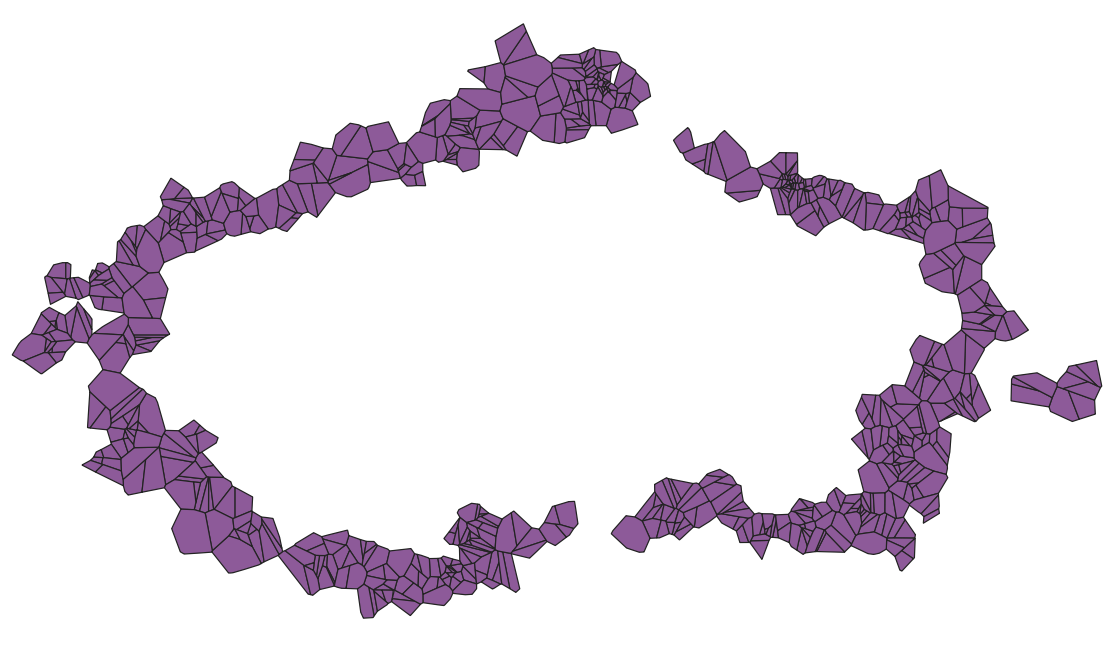
\includegraphics[width=400pt]{./pictures/voronoi-selected.png}
    \caption[Vybrané Voroného polygony pro pásmo 2]{Vybrané Voroného polygony pro pásmo 2}
	\label{fig:voronoi-selected}              
\end{figure}

Tyto polygony byly následně nástrojem \textit{Dissolve} spojeny do jednoho společného polygonu.
Vstupem tohoto nástroje byl výstup nástroje \textit{Select by location} a výstupem byl polygon
s jednou geometrií. 

\begin{figure}[H] \centering
    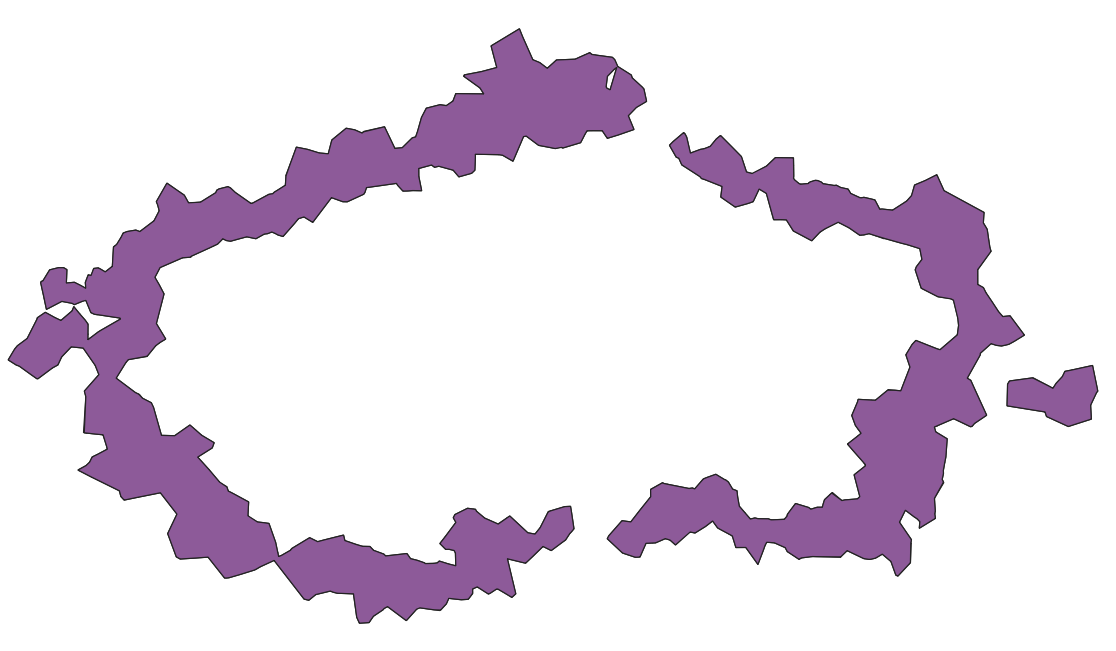
\includegraphics[width=400pt]{./pictures/dissolve.png}
    \caption[Výsledek nástroje Dissolve pro pásmo 2]{Výsledek nástroje Dissolve pro pásmo 2}
	\label{fig:dissolve}              
\end{figure} 

Kvůli mnoha zastávkám, které v oblasti pásem P, 0 a B v poli \textit{zone\_id} obsahovali hodnotu \textit{NULL},
vznikla uvnitř polygonu spousta mezer a děr. V těchto dírách dokonce někdy ležely i části malých polygonů, které 
avšak už po nástroji \textit{Dissolve} tvořili jeden celistvý polygon. A proto nebylo možné rovnou použít nástroj Delete holes,
nýbrž nejprve nástroj \textit{Multipart to singleparts}.

Nástroj \textit{Multipart to singleparts} rozdělil jeden vícedílný polygon na jednotlivé menší polygony. Vstupem do tohoto
nástroje je vektorová vrstva výstupu nástroje Dissolve a výstupem je vektorová vrstva s rozděleným polygonem.

Poté se pomocí metody \textit{selectByExpression} třídy \textit{QgsVectorLayer} vyhledal nej\-větší polygon
výrazem:

\[\$area = maximum(\$area, "zone\_id")\]

Takový polygon byl uložen do nové vektorové vrstvy. 

Poté již byl použit nástroj \textit{Delete holes}, který zaplnil vytvořené díry. Vstupem do tohoto nástroje byla vektorová
vrstva s největší polygonu z nástroje \textit{Dissolve}. Nástroj obsahoval volitelný parametr rozlohy, který byl
nastaven na hodnotu 500 a se kterým se nástroj \textit{Delete holes} řídí a zaplňuje menší díry, než je tento parametr.  

Znázornění tohoto postupu je zobrazeno zde v obrázku \ref{fig:postup-voronoi-P0B}. Toto zobrazení bylo provedeno v Grafickém modeláři.

\begin{figure}[H] \centering
    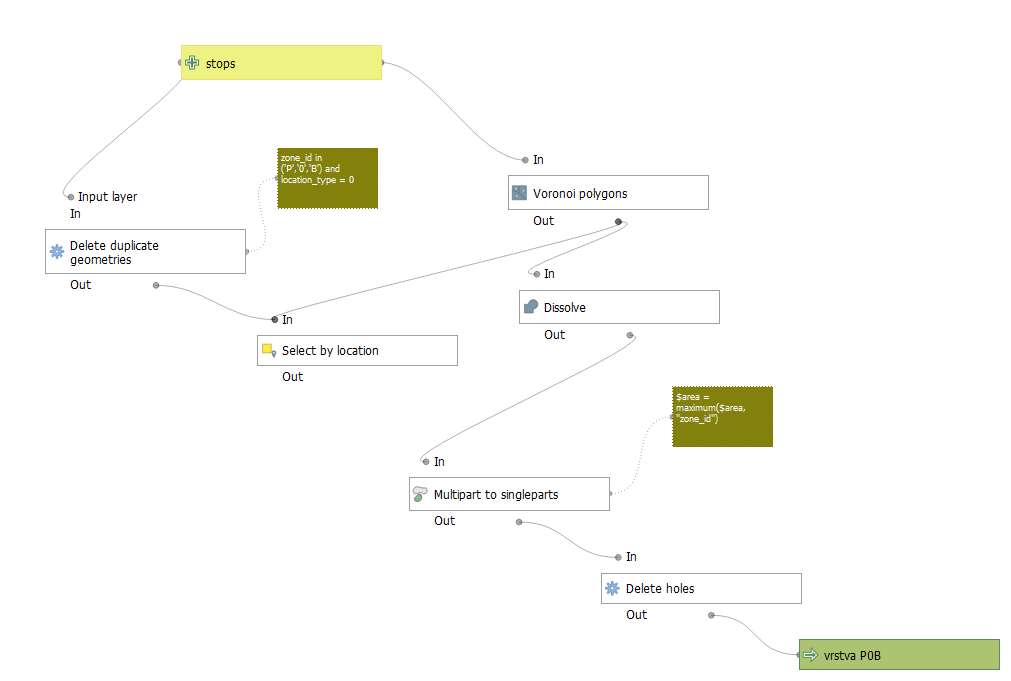
\includegraphics[width=400pt]{./pictures/postup-voronoi-P0B.png}
    \caption[Postup pro tarifní pásma P, 0 a B]{Postup pro tarifní pásma P, 0 a B}
	\label{fig:postup-voronoi-P0B}              
\end{figure}

\subsubsection{Tarifní pásma 1 až 9}
\label{tp_1az9}

Obdobný postup jako u tarifních pásem P, 0 a B, avšak znatelně jednodušší, byl proveden za pomocí
for cyklu pro tarifní pásma 1 až 9. 

Opět ty zástávky, které ležely v určitém pásmu, byly vyhledány pomocí metody \textit{selectByExpression} třídy 
\textit{QgsVectorLayer}. Pro zastávky tarifních pásem 1 až 6 to bylo provedeno pomocí dotazu:

\["zone\_id"\ <=\ "ID\: pasma"\ AND\ "zone\_id"\ !=\ '-'\ AND\ "location\_type" = 0\]  

Pro zastávky tarifních pásem 7 až 9 pomocí dotazu:
\["zone\_id"\ =\ "ID\: pasma"\ AND\ "location\_type" = 0\] 

V dotazu pro tarifní pásma 1 až 6 byly vybrány ty zastávky, které mají hodnotu pole \textit{zone\_id} menší jak aktuální hodnota,
hodnota pole \textit{zone\_id} se nerovná "pomlčce" (jelikož zastávky s touto hodnotou jsou mimo tarifní pásma)
a hodnota pole \textit{location\_type} byla rovna nule. V dotazu pro tarifní pásma 7 až 9 byly vybrány ty zastávky,
které mají hodnotu pole \textit{zone\_id} aktuální hodnotě a hodnota pole \textit{location\_type} byla rovna nule.

Důvodem pro dělení těchto dotazů byla jednak časová náročnost délky průběhu následujícího nástroje \textit{Select by location}, 
kde kvůli operátoru "<=" u dotazu pro zastávky tarifních pásem 1 až 6 do nástroje vstupují všechny zastávky, 
které jsou hodnotou ID menší jak aktuální hodnota. Tím se pro každé tarifní pásmo násobně zvětšuje počet zastávek,
které vstupují do nástroje \textit{Select by location}.

Pro tarifní pásma 7 až 9 byla časová náročnost stejná, jako u tarifních pásem P, 0 a B.

Hlavním důvodem avšak bylo "zalepení" děr, které vznikaly u vyhlazení tvaru tarifních pásem v kapitole \ref{vyhlazeni}.  

Následně byl pouze spuštěn \textit{Dissolve} pro spojení Voroného polygonů, což bylo vstupem do tohoto nástroje,
do jednoho celistvého polygonu, což bylo výstupem tohoto nástroje.

V následujícím obrázku \ref{fig:postup-voronoi-1az9} je souhrnně zobrazen postup tarifní pásma 1 až 9.

\begin{figure}[H] \centering
    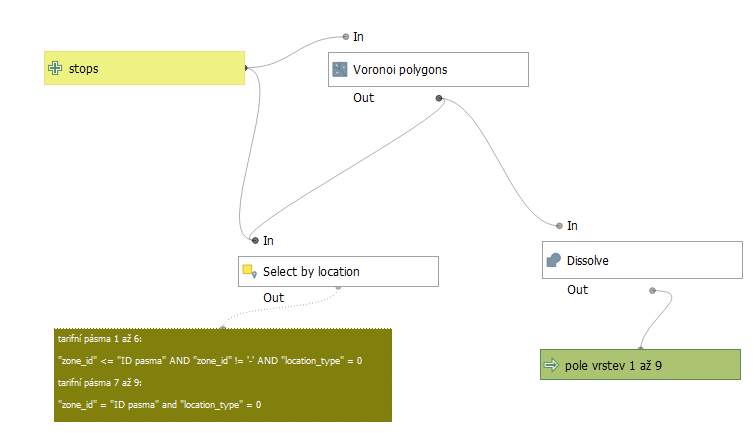
\includegraphics[width=400pt]{./pictures/postup-voronoi-1az9.png}
    \caption[Postup pro tarifní pásma 1 až 9]{Postup pro tarifní pásma 1 až 9}
	\label{fig:postup-voronoi-1az9}              
\end{figure}

\subsection{Vyhlazení tvaru tarifních pásem}
\label{vyhlazeni}

Pro vytvoření kartograficky přesných a vizuálně přijatelnějších tarifních pásem dosavadní postup nestačil.
V datasetu PID\_GTFS souboru \textit{stops.txt} existovaly takové zastávky, které měly tarifní pásmo sdílené
na rozhraní pásem. Těmito zastávkami měli podle pravidel ROPIDu tarifní pásma procházet.

Musel být navržen další průběh úpravy dosavadního tvaru tarifních pásem, který takovou podmínku zahrnuje
a zároveň vyhlazuje tvar polygonů pro lepší vizuální tvar.  

Ze spojených polygonů byla vygenerována vektorová vrstva bodů nástrojem
\textit{Extract vertices}, která představovala vrcholy spojených polygonů. Pro tuto vrstvu
bylo vstupem výstup nástroje \textit{Dissolve} a výstupem byl vektorová vrstva bodů 
doplněná o pole (mimo původních polí z vektorové vrstvy \textit{stops}) jako \textit{vertex\_index,
vertex\_part, vertex\_part\_ring, distance} a \textit{angle}.
Hodnoty těchto polí avšak nebyly využity v dalším výpočtu.

\begin{figure}[H] \centering
    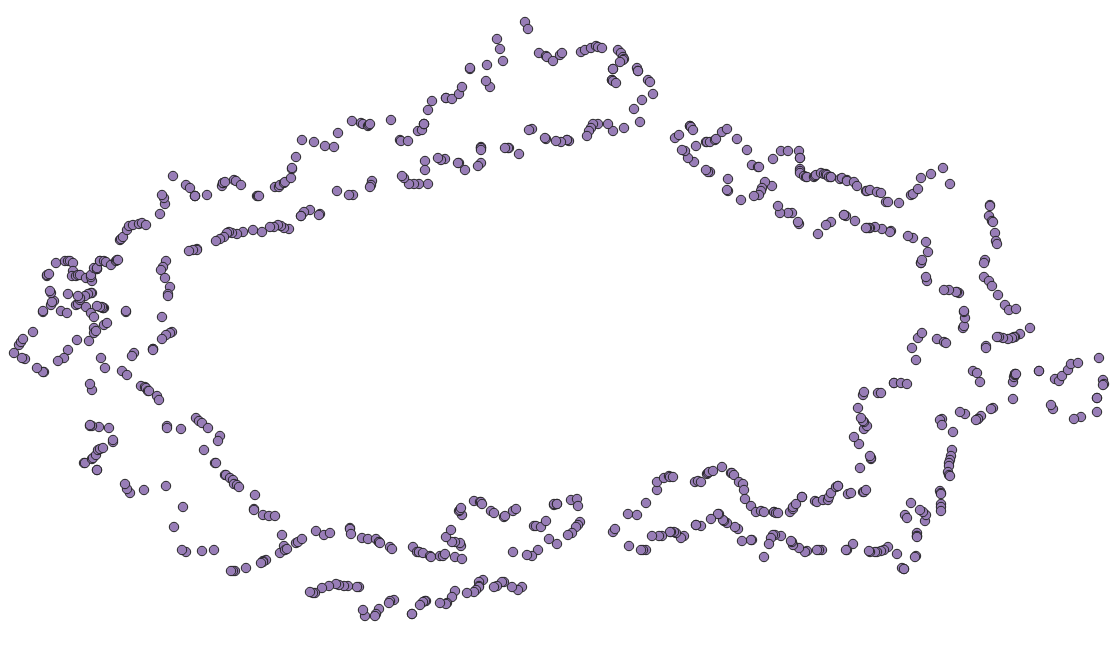
\includegraphics[width=400pt]{./pictures/vertices.png}
    \caption[Výsledek nástroje Extract vertices pro pásmo 2]{Výsledek nástroje Extract vertices pro pásmo 2}
	\label{fig:vertices}              
\end{figure} 

Dále byly s pomocí třídy \textit{QgsVectorLayer} a její metody \textit{selectByExpression} vybrány 
z původní vektorové vrstvy \textit{stops} ty zastávky, které ležely na hranici tarifních pásem.
Takové zastávky obsahovaly v poli \textit{zone\_id} hodnoty tarifních pásem oddělené čárkami.
Například pro zastávky mezi pásmem 1 a 2 byla hodnota pole "zone\_id" uvedena jako "1,2".

Pro tarifní pásma P, 0 a B byl použit dotaz:

\["zone\_id"\ NOT\ IN\ ('P',\ '0',\ 'B',\ '1',\ '2',\ '3',\ '4',\ '5',\ '6',\ '7',\ '8',\ '9')\]
\[("zone\_id"\ LIKE\ '\%P\%'\ OR\ "zone\_id"\ LIKE\ '\%0\%'\ OR\ "zone\_id"\ LIKE\ '\%B\%')\]

Pro tarifní pásma 1 až 9 byl použit dotaz:
\["zone\_id"\ LIKE\ "ID\: pasma\ i,ID\: pasma\ i+1"\]

Vybrané tarifní pásma byla uložena do nové vektorové vrstvy po následné i pozdější použití viz kapitola \ref{seskupeni}.

Následně byly pro každé tarifní pásmo byly spojeny vektorové vrstvy hraniční zastávek, 
zastávek uvnitř tarifního pásma a bodů z výstupu nástroje \textit{Extract vertices} nástrojem \textit{Merge vector layers}.
Tyto tři zmiňované vektorové vrstvy byly vstupem do tohoto nástroje a výstupem byla 
vektorová vrstva spojených bodů. 

\begin{figure}[H] \centering
    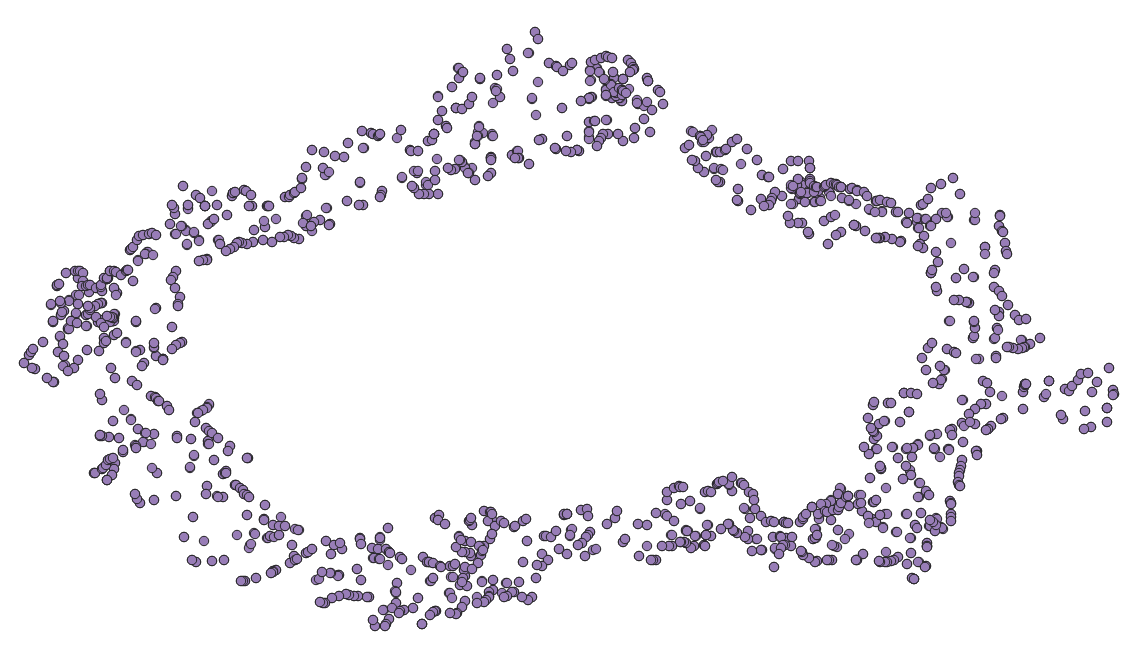
\includegraphics[width=400pt]{./pictures/merged.png}
    \caption[Spojené body třech vektorových vrstev pro pásmo 2]{Spojené body třech vektorových vrstev pro pásmo 2}
	\label{fig:merged}              
\end{figure} 

Pro spojení bodů a vytvoření jakési obálky byl nejdříve vyzkoušen nástroj \textit{Minimum bounding box} s možností Convex Hull,
což je aplikace algoritmu Konvexní obálky viz \ref{konv_obalka}. Tento způsob však velmi zjednodušoval tvar
tarifních pásem, a proto nástroj \textit{Minimum bounding box} nebyl použit.

Byla zvolena další možnost nástroje QGISu spojující body do jisté obálky. Tím nástrojem byl \textit{Concave hull (alpha shapes)} 
využívající aproximaci alpha-shapes viz kapitola \ref{konk_obalka}

Vstupem nástroje tedy byla vrstva spojených bodů, což byl první parametr
nástroje. Dalším parametrem byl práh (Threshold) s datovým typem \textit{čísla}, který byl volen od 0 do 1,
kdy 0 znamenala maximum konkávní obálky a 1 konvexní obálky. Po několika testovacích spuštění byla 
určena hodnota 0,09 jako nejlepší hodnotou pro tvorbu tarifních pásem. Dalším parametrem bylo Povolení děr (Allow holes) 
s datovým typem \textit{boolean}, který byl nastaven na \textit{False}.
Posledním parametrem bylo Rozdělit vícedílnou geometrii na jednotlivé části (Split multipart geometry 
into singlepart geometries) taktéž s datovým typem \textit{boolean}, který byl nastaven na \textit{True}.  
Výstupem byla polygonová vrstva konkávní obálky. 

Vytváření konkávní obálky bylo dalším důvodem pro dělení atributových dotazů v kapitole \ref{tp_1az9} pro 
zaplnění děr v tarifních pásmech 6 a nižších.  

\begin{figure}[H] \centering
    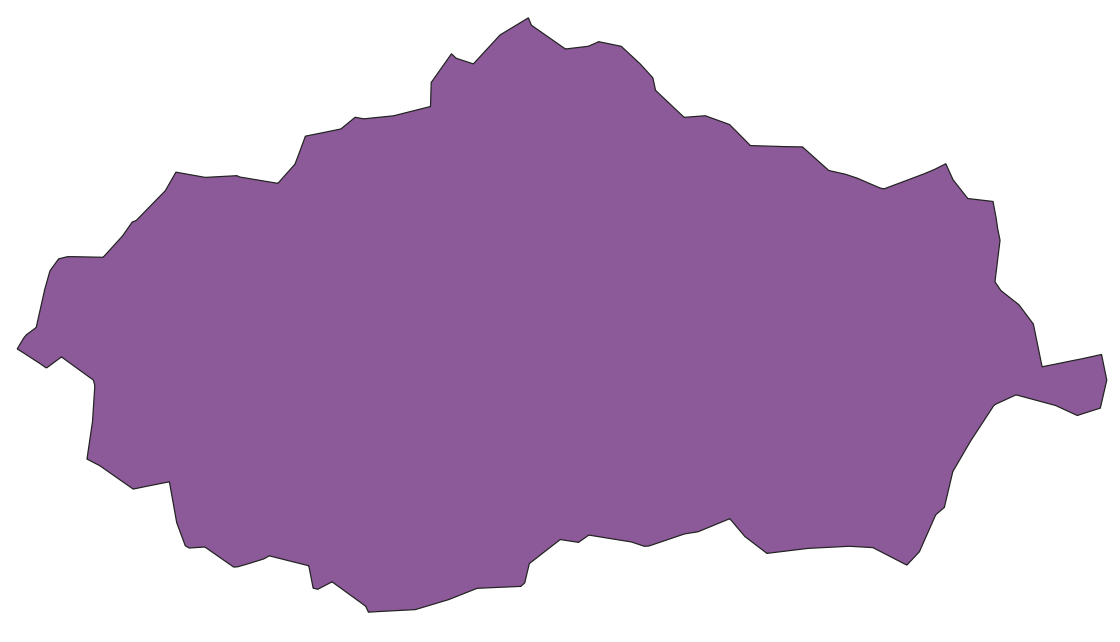
\includegraphics[width=400pt]{./pictures/concaveHull.png}
    \caption[Konkávní obálka pro pásmo 2]{Konkávní obálka pro pásmo 2}
	\label{fig:concaveHull}              
\end{figure} 

Z konkávní obálky byla pomocí nástroje Simplify "zjednodušena" geometrie polygonové vrstvy. Tento nástroj
využívá tři druhy zjednodušení vektorové vrstvy: založené na vzdálenosti (algoritmus „Douglas-Peucker“),
založené na ploše (algoritmus „Visvalingam“) a přichytávání geometrií k mřížce.
Pro můj postup byl zvolen první volba zjednodušení, pomocí algoritmu „Douglas-Peucker“ viz kapitola \label{generalizace_zjemneni}.

Do nástroje \textit{Simplify} byl vstupem výsledek nástroje \textit{Concave hull (alpha shapes)}, parametrem byl výběr algoritmu 
a nastavení hodnoty tolerance vzdálenosti. Výstupem byla polygonová vektorová vrstva.

\begin{figure}[H] \centering
    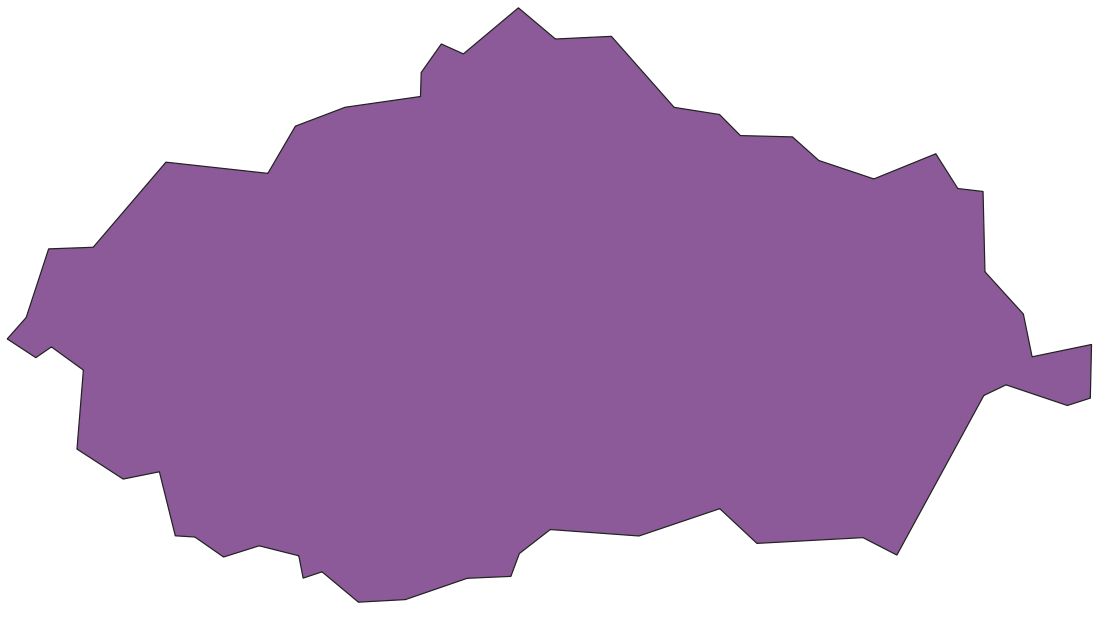
\includegraphics[width=400pt]{./pictures/simplify.png}
    \caption[Výsledek nástroje Simplify pro pásmo 2]{Výsledek nástroje Simplify pro pásmo 2}
	\label{fig:simplify}                                
\end{figure}

Výstup nástroje \textit{Simplify} byl vstupem do nástroje \textit{Smooth}. Tento nástroj vyhlazuje geometrie
liniové nebo polygonové vrstvy pomocí Chaikinova algoritmu viz kapitola \ref{vyhlazeni}.

U nástroje \textit{Smooth} byly zvoleny tři parametry - počet iterací, offset a maximální úhel.
Počet iterací znamená, kolik vyhlazovacích iterací bude použito pro každou geometrii.
Hodnota počtu iterací byla nastavena na 10, což byla maximální volitelná hodnota (pro co nevětší hladkost).
Parametr offset znamená, jak "těsně" vyhlazené geometrie sledují původní geometrie.
Zde byla ponechána výchozí hodnota 0,25. A poslední parametr maximálního úhlu lze použít
k zabránění vyhlazení uzlů s velkými úhly. Zde byla také ponechána výchozí hodnota 180°.
Výstupem nástroje byla polygonová vektorová vrstva.

\begin{figure}[H] \centering
    
\includegraphics[width=400pt]{./pictures/smooth.png}
    \caption[Výsledek nástroje Smooth pro pásmo 2]{Výsledek nástroje Smooth pro pásmo 2}
	\label{fig:smooth}                                
\end{figure}

Zde je souhrnně zobrazen postup této části pomocí Grafického modeláře na obrázku \ref{fig:postup-smooth}.

\begin{figure}[H] \centering
    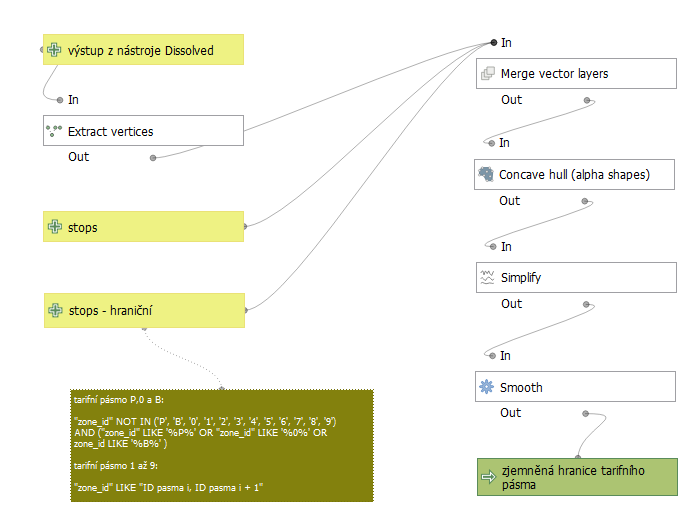
\includegraphics[width=400pt]{./pictures/postup-smooth.png}
    \caption[Postup pro zjemnění tvaru tarfních pásem]{Postup pro zjemnění tvaru tarfních pásem}
	\label{fig:postup-smooth}              
\end{figure}

\subsection{Hraniční tarifní pásma}

Jedním z největších problémů diplomové práce bylo se vypořádat s hraničním zastávkami.

\subsection{Seskupení tarifních pásem}
\label{seskupeni}

\subsection{Obarvení tarifních pásem}

\begin{figure}[H] \centering
    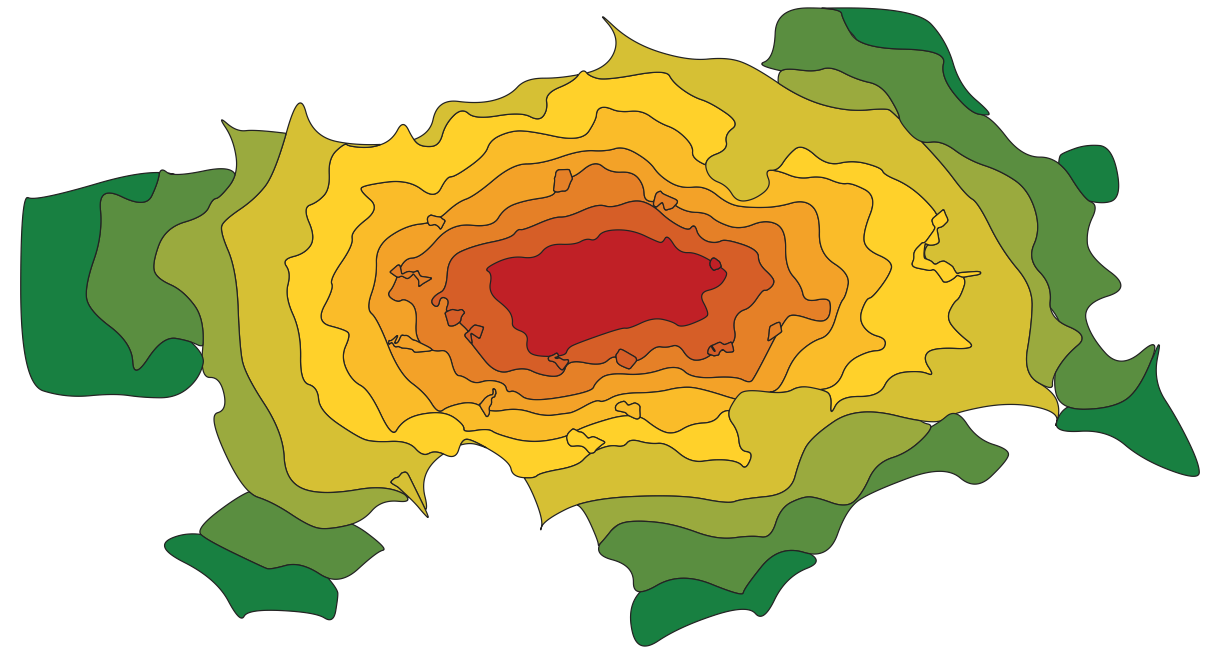
\includegraphics[width=400pt]{./pictures/vysledek.png}
    \caption[Výsledný tvar tarifních pásem]{Výsledný tvar tarifních pásem}
	\label{fig:vysledek}              
\end{figure}